% !TEX TS-program = pdflatexmk
\documentclass[a4paper,twoside,draft]{article}

\usepackage{epsfig}
\usepackage{subcaption}
\usepackage{calc}
\usepackage{amssymb}
\usepackage{amstext}
\usepackage{amsmath}
\usepackage{amsfonts}
\usepackage{amsthm}
\usepackage{multicol}
\usepackage{pslatex}
\usepackage{apalike}

\usepackage[scaled=0.8]{helvet}    % Less huge \textsf{functionName}
\usepackage[misc,geometry]{ifsym} % for letter symbol
\usepackage{soul}           % \hl for highlighting text; \st for strike-through
\usepackage{graphicx}
\usepackage[dvipsnames]{xcolor}
\usepackage{tikz}
\usetikzlibrary{trees,snakes,arrows}
\usetikzlibrary{shapes,chains}
\usetikzlibrary{positioning}
\usepackage{hyperref}
\usepackage[nospace]{cite}

\usepackage{SCITEPRESS}     % Please add other packages that you may need BEFORE the SCITEPRESS.sty package.

\usepackage{ifthen}

% -- Fonts and styles for names
\newcommand{\mFunStyle}[1]{\textsf{#1}}
\newcommand{\mConstStyle}[1]{\textsf{#1}}
\newcommand{\mVarStyle}[1]{\mathit{#1}}
\newcommand{\mFactStyle}[1]{\textsf{#1}}
\newcommand{\mMethodStyle}[1]{\mConstStyle{#1}}
\newcommand{\mProtocolStyle}[1]{\text{#1}}

% -- Macros for consistent wording
\newcommand{\mSpec}{specification}  % The EDHOC spec document we are analyzing

% -- Domain specific macros
\newcommand{\mArxiv}{\texttt{arXiv}}
\newcommand{\mTamarin}{\mProtocolStyle{Tamarin}}
\newcommand{\mProverif}{\mProtocolStyle{ProVerif}}
\newcommand{\mEdhoc}{\mProtocolStyle{EDHOC}}
\newcommand{\mOscore}{\mProtocolStyle{OSCORE}}
\newcommand{\mSigma}{\mProtocolStyle{SIGMA}}
\newcommand{\mSigmaI}{\mProtocolStyle{SIGMA\nobreakdash-I}}
\newcommand{\mCbor}{\mProtocolStyle{CBOR}}
\newcommand{\mCose}{\mProtocolStyle{COSE}}
\newcommand{\mCoseEncrypt}{\mProtocolStyle{COSE\_Encrypt0}}
\newcommand{\mCoseSign}{\mProtocolStyle{Cose\_Sign1}}
\newcommand{\mHkdf}{\mProtocolStyle{HKDF}}
\newcommand{\mHkdfExtract}{\mProtocolStyle{HKDF\nobreakdash-extract}}
\newcommand{\mHkdfExpand}{\mProtocolStyle{HKDF\nobreakdash-expand}}
\newcommand{\mHmac}{\mProtocolStyle{HMAC}}
\newcommand{\mAead}{\mProtocolStyle{AEAD}}
\newcommand{\mAeadDecrypt}{\mProtocolStyle{AEAD\nobreakdash-decrypt}}
\newcommand{\mDecrypt}{\mProtocolStyle{decrypt}}
\newcommand{\mOptls}{\mProtocolStyle{OPTLS}}
\newcommand{\mNoise}{\mProtocolStyle{Noise}}
\newcommand{\mTls}{\mProtocolStyle{TLS}}
\newcommand{\mDandTls}{\mProtocolStyle{(D)TLS}}
\newcommand{\mCtls}{\mProtocolStyle{cTLS}}
\newcommand{\mCoap}{\mProtocolStyle{CoAP}}

\newcommand{\mStat}{\mMethodStyle{STAT}}
\newcommand{\mSig}{\mMethodStyle{SIG}}
\newcommand{\mPsk}{\mMethodStyle{PSK}}
\newcommand{\mStatStat}{\mMethodStyle{STAT-STAT}}
\newcommand{\mStatSig}{\mMethodStyle{STAT-SIG}}
\newcommand{\mSigStat}{\mMethodStyle{SIG-STAT}}
\newcommand{\mSigSig}{\mMethodStyle{SIG-SIG}}
\newcommand{\mPskPsk}{\mMethodStyle{PSK-PSK}}

\newcommand{\mSid}{\mConstStyle{sid}}    % session id = (u, v, s-key)

\newcommand{\mXor}{\mConstStyle{XOR}}
\newcommand{\mSuites}{\mConstStyle{Suites\_I}}
\newcommand{\mMethod}{\mConstStyle{Method}}
\newcommand{\mCi}{\mConstStyle{C\_I}}
\newcommand{\mCr}{\mConstStyle{C\_R}}
\newcommand{\mGi}{\mConstStyle{G\_I}}
\newcommand{\mGr}{\mConstStyle{G\_R}}
\newcommand{\mGiy}{\mConstStyle{G\_IY}}
\newcommand{\mGrx}{\mConstStyle{G\_RX}}
\newcommand{\mGx}{\mConstStyle{G\_X}}
\newcommand{\mGy}{\mConstStyle{G\_Y}}
\newcommand{\mGxy}{\mConstStyle{G\_XY}}
\newcommand{\mIDPsk}{\mConstStyle{ID\_PSK}}
\newcommand{\mTH}{\mConstStyle{TH}}
\newcommand{\mTHtwo}{\mConstStyle{TH\_2}}
\newcommand{\mKtwoe}{\mConstStyle{K\_2e}}
\newcommand{\mKtwom}{\mConstStyle{K\_2m}}
\newcommand{\mKtwoae}{\mConstStyle{K\_2ae}}
\newcommand{\mSign}{\mConstStyle{sign}}

\newcommand{\mKthreeae}{\mConstStyle{K\_3ae}}
\newcommand{\mKthreem}{\mConstStyle{K\_3m}}

\newcommand{\mTHthree}{\mConstStyle{TH\_3}}
\newcommand{\mhplain}{\mConstStyle{h''}}
\newcommand{\mCredi}{\mConstStyle{CRED\_I}}
\newcommand{\mCredr}{\mConstStyle{CRED\_R}}
\newcommand{\mHash}{\mConstStyle{H}}

\newcommand{\mTHfour}{\mConstStyle{TH\_4}}
\newcommand{\mAuthi}{\mConstStyle{Auth\_I}}
\newcommand{\mAuthr}{\mConstStyle{Auth\_R}}

\newcommand{\mMactwo}{\mConstStyle{MAC\_2}}
\newcommand{\mMacthree}{\mConstStyle{MAC\_3}}

\newcommand{\mSigtwo}{\mConstStyle{Sig\_2}}
\newcommand{\mSigthree}{\mConstStyle{Sig\_3}}

\newcommand{\mMsgone}{\mConstStyle{m1}}
\newcommand{\mMsgtwo}{\mConstStyle{m2}}
\newcommand{\mMsgthree}{\mConstStyle{m3}}

\newcommand{\mCipher}{\mConstStyle{cipher\_2}}

\newcommand{\mAD}{\mConstStyle{AD}}
\newcommand{\mADone}{\mConstStyle{AD\_1}}
\newcommand{\mADtwo}{\mConstStyle{AD\_2}}
\newcommand{\mADthree}{\mConstStyle{AD\_3}}

\newcommand{\mPRK}{\mConstStyle{PRK}}
\newcommand{\mPRKtwo}{\mConstStyle{PRK\_2e}}
\newcommand{\mPRKthree}{\mConstStyle{PRK\_3e2m}}
\newcommand{\mPRKfour}{\mConstStyle{PRK\_4x3m}}

\newcommand{\mIdcredi}{\mConstStyle{ID\_CRED\_I}}
\newcommand{\mIdcredr}{\mConstStyle{ID\_CRED\_R}}
\newcommand{\mLtki}{\mConstStyle{ltk\_I}}
\newcommand{\mLtkr}{\mConstStyle{ltk\_R}}
\newcommand{\mLtk}{\mConstStyle{ltk}}

% TIKZ messages and actions
\newcommand{\msg}[4]{\draw[->,thick] ([yshift=-#1]#2.south) coordinate (l1)--(l1-|#3) node[midway, above]{#4}}
\newcommand{\action}[3]{\node[draw,thick,fill=white,align=center,below={#1} of {#2}]{#3}}

% Tamarin symbols
\newcommand{\ifarrow}[1]{\ensuremath{\mathit{\,-\hspace{-2.4pt}[{#1}]\hspace{-4.95pt}\rightarrow\,}}}
\newcommand{\semarrow}[1]{\ensuremath{\mathit{\,=\hspace{-4.9pt}[{#1}]\hspace{-5pt}\Rightarrow\,}}}
\newcommand{\mIn}{\mathsf{In}}
\newcommand{\mOut}{\mathsf{Out}}
\newcommand{\mFr}{\mathsf{Fr}}
\newcommand{\mKD}{\mathsf{KD}}
\newcommand{\mKU}{\mathsf{KU}}
\newcommand{\mT}[1]{\lstinline[basicstyle=\sffamily\normalsize]{#1}} % Tamarin code inline
\usepackage[final]{listings}

\lstdefinestyle{mystyle}{
    backgroundcolor=,   
    commentstyle=\color{Green},
    identifierstyle=\color{black},
    keywordstyle=\color{ForestGreen},
    numberstyle=\color{Gray},
    stringstyle=,
    basicstyle=\sffamily\small,
    keywords={let,in,rule,restriction,axiom,lemma,all-traces,exists-trace,Ex,All,Fr,In,Out},
    breakatwhitespace=false,
    breaklines=true,
    captionpos=b,
    keepspaces=false,
    numbers=left,
    numbersep=5pt,
    showspaces=false,
    showstringspaces=false,
    showtabs=false,
    tabsize=2,
    morecomment=[l]{//},
    literate=
    {=}{$=$}{1}
    {[}{$[$}{1}%
    {]}{$]$}{1}%
    {<}{$\langle$}{1}%
    {>}{$\rangle$}{1}%
    {(}{$($}{1}%
    {)}{$)$}{1}%
    {&}{$\wedge$}{1}
    {|}{$\vee$}{1}
    {$}{\$}{1}
    {<\ \#}{$<$\ \ \#}{3}% trick here: we distinguish angle brackets from temporal comparisons because of the # for the variable on the rhs
    {--[}{$\mbox{-\hspace{-4.0pt}[}$}{3}%
    {]->}{$\mbox{]\hspace{-4.2pt}\rightarrow}$}{3}%
    {-->}{$\rightarrow$}{1}
    {==>}{$\Rightarrow$}{1}
    {XOR}{$\oplus$}{1}%
    {aeadEncrypt}{\mAead{}}{6}%
    {decrypt}{\mDecrypt}{6}
    {aeadDecrypt}{\mAeadDecrypt}{11}
    {hkdfExtract}{\mHkdfExtract}{14}
    {hkdfExpand}{\mHkdfExpand}{14}
    {All\ }{$\forall$\ }{3}
    {Ex\ }{$\exists$\ }{3}
    {h(}{H$($}{2}
    {~}{{\url{~}}}{1}
    }
\lstset{style=mystyle}


\begin{document}
\title{Formal Analysis of EDHOC Key Establishment for Constrained IoT Devices}
% \author{Karl Norrman\inst{1,2}\textsuperscript{(\Letter)}\orcidID{0000-0003-0164-1478}
% \and
%     Vaishnavi Sundararajan\inst{3}
% \and
%     Alessandro Bruni\inst{4}
% }
\author{
    \authorname{
        Karl Norrman\sup{1,2}%\orcidAuthor{0000-0003-0164-1478}
        , Vaishnavi Sundararajan\sup{3} and
        Alessandro Bruni\sup{4}
    }
    %
    \affiliation{\sup{1}KTH Royal Institute of Technology, Stockholm, Sweden}
    \affiliation{\sup{2}Ericsson Research, Security, Stockholm, Sweden}
    \affiliation{\sup{3}University of California Santa Cruz, USA}
    \affiliation{\sup{4}IT University of Copenhagen, Copenhagen, Denmark}
    %
    \email{karl.norrman@ericsson.com, vasundar@ucsc.edu, brun@itu.dk}
}
%\author{}

\keywords{Formal Verification, Symbolic Dolev-Yao Model,
          Authenticated Key Establishment, Protocols, IoT.}

\abstract{
Constrained IoT devices are becoming ubiquitous in society
and there is a need for secure communication protocols that respect the
constraints under which these devices operate.
%
\mEdhoc{} is an authenticated key establishment protocol for constrained IoT
devices, currently being standardized by the Internet Engineering Task
Force (IETF).
%
A rudimentary version of \mEdhoc{} with only two key establishment methods was
formally analyzed in 2018.
%
Since then, the protocol has evolved significantly and several new key
establishment methods have been added.
%
In this paper, we present a formal analysis of all \mEdhoc{} methods in an
enhanced symbolic Dolev-Yao model using the \mTamarin{} tool.
%
We show that not all methods satisfy the authentication notion
injective agreement, but that all do satisfy a notion of implicit
authentication, as well as Perfect Forward Secrecy (PFS) of the session key material.
%
We identify other weaknesses to which we propose improvements
%
For example, a party may intend to establish a session key with a certain peer,
but ending up establishing it with another, trusted but compromised, peer.
%
We communicated our findings and proposals to the IETF, which
has incorporated some of these in newer versions of the standard.
}
%

\onecolumn \maketitle \normalsize \setcounter{footnote}{0} \vfill
%-------------------------------------------------------------------------- sec
\section{\uppercase{Introduction}}
\label{sec:introduction}

%-------------------------------------------------------------------------- sub
%\subsection{Background and motivation}
%\label{sec:motivation}
As IoT devices become more prevalent and get involved in progressively sensitive
functions in society, the need to secure their communications
becomes increasingly important.
%
Most of the security analysis of IoT devices have focused on computationally
strong devices, such as cars and web-cameras, where existing protocols like
\mDandTls{} suffice.
%
Constrained devices, on the other hand, which operate under severe
bandwidth and energy consumption restrictions, have received much less
attention.
%
These devices may be simple sensors which only relay environment
measurements to a server every hour, but need to function autonomously without
maintenance for long periods of time.
%
The IETF standardized the Object Security for
Constrained RESTful Environments (\mOscore{}) protocol to secure communications
between constrained devices~\cite{rfc8613}.
%
However, the \mOscore{} protocol requires a pre-established security context.
%
The IETF has been discussing requirements and mechanisms for a key
exchange protocol, named Ephemeral Diffie-Hellman Over COSE (\mEdhoc), for
establishing \mOscore{} security contexts.
%
Naturally, \mEdhoc{} must work under the same constrained requirements as
\mOscore{} itself.
%
While not all use cases for \mEdhoc{} are firmly set, the overall goal is to
establish an \mOscore{} security context, under message size limitations.
%
It is therefore important to ensure that \mEdhoc{} satisfies fundamental
security properties expected from a key exchange protocol.
%The work is now being done in the IETF Lightweight Authenticated Key Exchange
%(LAKE) working group.
%

The first incarnation of \mEdhoc{} appeared in March 2016.
%
It contained two different key establishment methods, one based on a
pre-shared Diffie-Hellman (DH) cryptographic core%
\footnote{By a \emph{cryptographic core}, or simply core, we mean an academic protocol,
without encodings or application specific details required by an industrial
protocol.
%
By a \emph{key establishment method} we mean a core with some such details added.
}
and a second based on a
variant of challenge-response signatures in the style of 
\mOptls{}~\cite{DBLP:conf/eurosp/KrawczykW16}.
%
\mEdhoc{} is therefore a framework of several key establishment methods.
%
In May 2018, the core based on challenge-response signatures was replaced by
one based on \mSigma{} (SIGn-and-MAc)~\cite{bruni-analysis-selander-ace-cose-ecdhe-08}.
%
Since then the protocol has undergone significant changes.
%
Three new cores, mixing challenge-response signatures and regular signature for
authentication, were added~\cite{our-analysis-selander-lake-edhoc-00}.
%

We formulate and formalize a security model covering all four key
establishment methods, which is important especially since the
\mSpec{}~\cite{our-analysis-selander-lake-edhoc-00} lacks a clear description
of the intended security model and overall security goals.
%
We perform the analysis in a symbolic Dolev-Yao model.
In this framework, we model messages as terms in an algebra, with operations such
as encryption, modelled as functions on these terms.
These functions are assumed perfect, e.g., one cannot decrypt an encrypted
message without access to the key.
The adversary, while unable to break encryption or reverse hashing, is modelled
as the network.
That is, the adversary, can block reroute, replay and modify messages at will.
A symbolic model like this, while slightly severe an abstraction, still allows
us to analyze \mEdhoc{} for logical flaws without incurring the complexity of
a computational model.
%
The standardization process is ongoing, with the authors releasing newer
versions of the \mSpec{} (see Section~\ref{sec:newdrafts} for more detail
about how these versions differ from the one analyzed here).
%

%-------------------------------------------------------------------------- sub
\subsection{Contributions}
\label{sec:contributions}
In this paper, we formally analyze the \mEdhoc{} protocol (with its four key
establishment methods) using the \mTamarin{} tool~\cite{DBLP:conf/cav/MeierSCB13}.
%
We present a formal model we constructed of the protocol as given in the
\mSpec{}~\cite{our-analysis-selander-lake-edhoc-00}.
%

We give an explicit adversary model for the protocol and verify
properties such as session key material and entity authentication, and perfect
forward secrecy, for all four methods.
%

The model itself is valuable as a basis for verifying further updates in the
ongoing standardization.
%
It is publicly available~\cite{edhocTamarinRepo}.
%
It took several person-months to interpret the
specification and construct the model.
%
Termination requires a hand-crafted proof oracle to guide \mTamarin{}.
%

We show that not all \mEdhoc{}'s key establishment
methods provide authentication according to the injective agreement definition
on the session key material, and none on the initiator's identity.
%
However, we show that all methods fulfill an implicit agreement property on
the session key material and the initiator's identity.
%
We identify a number of subtleties, ambiguities and weaknesses in the
specification.
%
For example, the authentication policy requirements allows situations where a
party establishes session key material with a trusted but compromised peer, even
though the intention was to establish it with a different trusted party.
%
We provide remedies for the identified issues and have
communicated these to the IETF and the specification authors, who incorporated
some of our suggestions and currently consider how to deal with the remaining
ones.
%

\subsection{Comparison with Related Work}
The May 2018 version of \mEdhoc{} was formally analyzed by
Bruni et~al.~\cite{DBLP:conf/secsr/BruniJPS18} using the \mProverif{}
tool~\cite{DBLP:conf/csfw/Blanchet01}.
%
Their analysis covered a pre-shared key authenticated core and one
based on \mSigma.
%
The properties checked for therein were secrecy, PFS and integrity of
application data, identity protection against an active adversary,
and strong authentication.
%

In contrast to the key establishment methods analyzed by Bruni et~al., which
were based on the well-understood pre-shared key DH and \mSigma{} protocols,
the three newly added
methods combine two unilateral authentication protocols with the goal to
constructing mutual authentication protocols.
%
Combining two protocols, which individually provide unilateral authentication,
is not guaranteed to result in a secure mutual authentication
protocol~\cite{DBLP:conf/ccs/Krawczyk16}.
%
Consequently, although the framework is similar to the one analyzed by Bruni
et~al., the cryptographic underpinnings have increased in complexity more than
twofold, and is using mechanisms which have not previously been formally analyzed.
%
The set of properties we check for is also different.
%
Our analysis is further carried out using a different tool,
namely \mTamarin; different kinds of strategies to formulate and
successfully analyze the protocol are required when working with this tool.
%

%-------------------------------------------------------------------------- sec
\section{\uppercase{The \mEdhoc{} Protocol}}
\label{sec:edhoc}
% !TEX root =  main.tex

%Description of \m\mEdhoc and main changes from last verified version

\vnote{I find the macros for the protocol, method, and tool names distracting while reading through (the font changes too much, too often). The macro for EDHOC actually inserts a line break if you start a sentence with it, because of the \texttt{hbox} (I'm not sure why the hbox exists for what is a macro to be inserted in running text). I do need to start sentence with EDHOC many times though, so this is irritating. It is also the case that ProVerif needs to be written like so, and not capitalized entirely, so at least one of them is plain wrong! For now I've left in the macros, but I'd prefer that we fixed them to be regular capitalized text or, in the case of ProVerif, in camelcase as they should be.}

\subsection{Overview}
Constrained IoT systems often deal with a lot of valuable personal and business information that ought to be kept secure. Such systems need to be assured of end-to-end protection with source authentication and perfect forward secrecy. It is often desirable to protect such devices at the application layer -- for example, in cases where transport layer security is not sufficient [\mcneed], or where multiple underlying protocols need to be accounted for. One method for providing application layer security is provided by CBOR Object Signing and Encryption (COSE) [RFC8152: \mcfix].  

In order to derive shared key material with which to proceed, communicating parties can run an Elliptic Curve Diffie-Hellman key exchange protocol with ephemeral keys. Ephemeral Diffie-Hellman Over COSE (\mEdhoc) is a lightweight key exchange protocol for such situations, and is expected to provide perfect forward secrecy and identity protection. \mEdhoc supports authentication using pre-shared keys (PSK), raw public keys (RPK), and public key certificates. After successful completion of the \mEdhoc protocol, application keys and other application specific data can be derived using the \mEdhoc-Exporter interface. 

A main use case for \mEdhoc is to establish a security context for Object Security for Constrained RESTful Environments (\mOscore) [RFC8613: \mcfix]. \mOscore is a protocol which uses COSE for application-layer protection on top of the transport-layer Constrained Application Protocol (CoAP). \mEdhoc uses COSE for cryptography, CBOR for encoding, and CoAP for transport. By reusing existing libraries, the additional code footprint can be kept very low.

\mEdhoc is designed to work in highly constrained scenarios. This makes it especially suitable for network technologies which have low throughput, low power consumption, and small frame sizes. Examples include Cellular IoT, 6TiSCH, and LoRaWAN [\mcneed].

\subsection{Background, comparison with~\cite{DBLP:conf/secsr/BruniJPS18}}
The first version of \mEdhoc was proposed in March 2016 to a working group investigating lightweight authenticated key exchange protocols [\mcneed]. There has been a focus on formally verifying that the protocol satisfies the properties expected of it right from the beginning. 

The 2018 work~\cite{DBLP:conf/secsr/BruniJPS18} by Bruni et al performed a formal verification of version 08 [\url{https://tools.ietf.org/html/draft-selander-ace-cose-ecdhe-08} \mcfix] of \mEdhoc. The protocol and properties are modelled and verified in the \mProverif tool. This version of the protocol belongs to the \mSigmaI family of protocols, and has two modes -- one with asymmetric keys, and one with pre-shared symmetric keys (PSK). Bruni et al showed that this version satisfies the requisite properties of identity protection, (perfect forward) secrecy of data, and strong authentication, upon completion of the protocol.

\mEdhoc has undergone a lot of change since version 08, as will be described in the following sections, and the formal verification of the current version, therefore, is a worthwhile exercise.

%\subsection{Overarching goal of security context establishment}
\subsection{Methods and features of \textsc{EDHOC}}
\mEdhoc can established Diffie-Hellman key exchange in one of three different ways -- using digital signatures, static Diffie-Hellman keys, or pre-shared symmetric keys. We describe each of these methods in detail below. The communicating parties must agree on the method as part of the first message.

\subsubsection{\mSigSig method}
The \mSigma (SIGn-and-MAc) family of protocols [\mcneed] has many variants. The \mSigSig method of \mEdhoc is built on \mSigmaI, a variant of the \mSigma protocol which provides identity protection for the initiator, and  implements the \mSigmaI variant as Mac-then-Sign. The current \mSigSig method corresponds (with a few minor changes) to the asymmetric key mode of \mEdhoc v08. 

The communicating parties exchange ephemeral public keys, compute the shared secret, and derive symmetric application keys from this secret.

\subsubsection{\mPskPsk method}
In this method, the initiator and responder are assumed to have a pre-shared key which is secret to them, and can be retrieved by the responder using a public part of the first message (\mIDPSK). This method corresponds to the symmetric key method of \mEdhoc v08. 

In the first message, the initiator sends a message consisting of the method name, the initiator's ephemeral key (\mGx), their connection identifier (\mCi), the \mIDPSK identifier, and (optional) plaintext (\mADone). 

The second message, sent by the responder, is composed of \mCi, the responder's ephemeral key \mGy, their connection identifier \mCr, and an AEAD encryption [\mcneed] of the transaction hash of the first message (\mTHtwo) along with an optional plaintext \mADtwo. The key used for this (\mKtwo) is derived using the EDHOC key derivation function with \mTHtwo and the pseudorandom string \mPRKtwo as input, while the associated data for the AEAD encryption is constructed by concatenating a constant string, the hash function, and \mTHtwo. 

The initiator, upon receipt of this message, sends back \mCr, followed by an AEAD encryption of the transaction hash of the second message (\mTHthree) along with a plaintext \mADthree. As earlier, the key used is derived by supplying \mTHthree and \mPRKthree as input to the KDF, and the  associated data obtained by concatenating the constant string, hash function, and \mTHthree. An abstract description is shown in Figure~\ref{fig:edhocpsk}.

\vnote{Figure numbers don't square up, check class file guidelines!}

\begin{figure}\label{fig:edhocpsk}
\centering
\includegraphics[scale=0.3]{Images/psk.png}
\caption{The PSK-PSK method of EDHOC}
\end{figure}

\subsubsection{\mStat-based methods}
\mEdhoc allows for three \mStat-based methods -- two where only one participant has a static Diffie-Hellman key (while the other uses signatures), and one where both do. This set of methods is not covered in v08 of \mEdhoc, which only has a single \mSigma asymmetric key method (corresponding to the \mSigSig method shown above). This allows one party to use a \mSigma style of authentication, while the other can use something along the lines of \mOptls.

\vnote{Need to talk about links to OPTLS and NOISE}



\subsection{Expected security properties}


%Discussion of KDF -- page 13 of EDHOC

%certain security applications may be integrated into EDHOC by transporting auxiliary data together with the messages. One example is the transport of third-party authorization information protected outside of EDHOC [I-D.selander-ace-ake-authz]. Another example is the embedding of a certificate enrolment request or a newly issued certificate. EDHOC allows opaque auxiliary data (AD) to be sent in the EDHOC messages. Unprotected Auxiliary Data (AD_1, AD_2) may be sent in message_1 and message_2, respectively. Protected Auxiliary Data (AD_3) may be sent in message_3. Since data carried in AD1 and AD2 may not be protected, and the content of AD3 is available to both the Initiator and the Responder, special considerations need to be made such that the availability of the data a) does not violate security and privacy requirements of the service which uses this data, and b) does not violate the security properties of EDHOC. 



%-------------------------------------------------------------------------- sec
\section{\uppercase{Formalization and Results}}
\label{sec:formalization}
Next we describe our approach at formalizing the \mEdhoc protocol. We use the
symbolic (Dolev-Yao) model for verification, using \mTamarin for tool support.
%
The next three subsections describe our threat model, briefly present the
\mTamarin tool, and our modeling choices.
%
Finally, we present the properties that we proved in this effort.

\subsection{Threat model}
We verify \mEdhoc in the symbolic Dolev-Yao model: as customary in this style of
modeling, we assume all cryptographic primitives to be ``perfect'', and hence
only allow the attacker to encrypt and decrypt messages when they know the key,
and exclude hash collisions, for example; the attacker is also in control of the
communication channel, and can interact with unbounded sessions of the protocol,
dropping, injecting and modifying messages at their liking.

One important point here is that we allow the attacker to impersonate malicious
endpoints, by revealing their long-term and session key material at any given
point.
%
\mEdhoc should remain secure under these assumptions, as we detail below.

\paragraph{Post-compromise security}
Post-compromise security is a class of properties that relate to the ability of
a protocol to maintain security of previous and future sessions under a
compromise.
%
Cohn-Gordon et al.~\cite{cohn2016post} present a formal characterization of this
class of properties.
%
In this paper we adopt their terminology, hence we refer to them for a detailed
explanation.

Briefly speaking,~\cite{cohn2016post} defines the \emph{classical adversary
  model} as the model that considers only sessions ran by honest parties; other
parties may be dishonest and thus reveal their private information to the
attacker, however the honest parties remain honest.
%
Under the classical model security must be maintained for the parties
considered.
%
\emph{Perfect forward secrecy} (PFS) drops the assumption that the parties
involved in the sessions considered shall remain honest: hence long-term key
material may be leaked after the run of a session, but such session must remain
secure.
%
Further, \emph{key-compromise impersonation} (KCI) takes the perspective of one
of the endpoints of the protocol, say Alice running a session with Bob. A
protocol is secure under KCI if Alice can still establish a secure session with
Bob, even though Alice's keys are compromised at any time, and Bob's key
material is not leaked until the end of the session.
%
Finally, \emph{weak} and \emph{strong post-compromise security} (PCS) consider
only those sessions run by parties that are not under control of the
attacker. These same parties can be under the attacker's control even before and
after the session.
%
A protocol with \emph{weak PCS} must guarantee security under a limited
compromise, where the key material is not leaked, but the attacker has access to
the compormised party to perform cryptographic operations (e.g. through
interfacing with a trusted computing module).
%
A protocol with \emph{strong PCS} gurantees security even if the attacker has
complete access to the state of both parties involved, up until before the
execution of the session under consideration and even after.
%
This is usually achieved by maintaining some state and performing key rotations,
hence the attacker must be able to observe the internal state of the device as
the protocol runs.
%
\emph{We do not check strong PCS} for \mEdhoc, as it is not secure under these
assumptions.

\paragraph{Session independence}
Finally we model \emph{session independence} of \mEdhoc, that is, we allow
leakage of session key material, and additionally check security only of those
sessions for which the session key material has not been revealed. We check this
in conjunction with PCS properties.

\subsection{Tamarin}
We chose \mTamarin to model and verify \mEdhoc in the Symbolic model.
%
\mTamarin is an interactive verification tool based on multi-set rewriting rules
with event annotations, which allows to check LTL temporal formulas on these
models.
%
Multi-set rewrite rules with events take the form:
%
\[ l \ifarrow[e] r \]
%
where $l$ and $r$ are multi-sets of facts, and $e$ is a multi-set of events.
%
Facts are $n$ary predicates over a term algebra, which defines a set of function
symbols $\mathcal F$, variables $\mathcal V$ and names $\mathcal N$. Tamarin
checks equality of thse terms under an equational theory $E$, hence one can
write that
%
\[ dec(enc(x,y),y) =_E x \]
%
to denote that symmetric decryption reverses the encryption operation, and so
forth. All operations on terms are defined under $E$, hence we omit the
subscript from now on as the equational theory is fixed per model.

\paragraph{Semantics and built-ins} On a first approximation, \mTamarin states
$S$, $S'$ are multisets of facts, and a semantic transition $S \semarrow[E] S'$
occurs if there is a rule $l \ifarrow[e] r$ and a substitution $\sigma$ such
that $S \supseteq \sigma(l)$ and $S' = S \setminus \sigma(l) \uplus \sigma(r)$
and $E = \sigma(e)$.

There are a few more details, such as persistent facts that are denoted by a $!$
and are never removed from the state.
%
The sorts fresh (denoted by $\sim$) and public (denoted by $\$$) denote fresh
constants and public values known to the attacker respectively, and are both
sub-sorts of a base sort.
%
Finally, \mTamarin has some built-in predicates ($\mIn,
\mOut$ to represent input and output of messages with the attacker, among
others), rules and equations that represent the attacker's knowledge and
standard equational theories in the symbolic model, plus syntactic sugar, all of
which we introduce as we see necessary.

For example in our model we have a symbol to denote authenticated encryption and
hence \mTamarin produces the rule:
%
\[ !\mKU( k ), !\mKU( m ), !\mKU( ad ), !\mKU( al ) \ifarrow !\mKU( \mAeadEncrypt(k, m, ad, al) ) \]
%
to denote that if the attacker knows a key $k$, a message
$m$, the authenticated data $ad$, and an algorithm
$al$, then they can construct the encryption using these parameters, hence get
to know the message $\mAeadEncrypt(k, m, ad, al)$.
%
There are two built-in persistent facts to denote attacker knowledge,
$!\mKU$ and
$!\mKD$, but we ignore their distinction for now as it is only necessary for
\mTamarin's termination properties.

In our model we introduce a theory for authenticated encryption, plus the
built-in theories of XOR and Diffie-Hellmann.
%
Authenticated encryption, which is encryption with authentication data as
detailed in~\cite{aead}, has the following two equations:
\begin{align*}
  \mAeadDecrypt(k, \mAeadEncrypt(k, m, ad, al), ad, al) = m\\
  \mDecrypt(k, \mAeadEncrypt(k, m, ad, al), al) = m
\end{align*}
With the first rule we allow the protocol to decrypt the message $m$ if the
encryption has matching key $k$, authenticated data $ad$, and uses the same
algorithm $al$.
%
The second rule allows the attacker to decrypt the message $m$ with the key $k$
and without the authenticated data $ad$, and hence skip the check.

The built-in theories for XOR and Diffie-Hellman are a fair bit more complex
than authenticated encryption, hence we refer to the original
papers~\cite{xorTamarin,dhTamarin} for a full reference.
%
Suffices to say that the XOR theory introduces the symbol $\oplus$, for
expressing XOR operations $x \oplus y$, plus the necessary equational theory
including associativity, commutativity, and inverse.
%
The theory for Diffie-Hellman introduces exponentiation $x^y$ and product
$x \cdot y$ as a built-in symbols in the language, plus the necessary equational
theory of associativity, commutativity, distributivity of exponentiation with
product, and inverse.

\subsection{Modeling \mEdhoc}
In this section we detail the modeling choices that we have made for this formal
verification effort.
%
We model the five different modes of \mEdhoc from a single specification
according to the five different combinations of authentication methods:
\mPskPsk, \mSigSig, \mSigStat, \mStatSig and \mStatStat.
%
We use the M4 macro language to derive these different modes from a single
description of the protocol, thus enforcing uniformity in the presentation.
%


\subsection{Properties}

%-------------------------------------------------------------------------- sec
\section{\uppercase{Discussion}}
\label{sec:discussion}
There are a few places where \mEdhoc{} can be improved,
which we found during this work and communicated to the authors.
%
We discuss them below.
%

%-------------------------------------------------------------------------- sub
%\subsection{Security Claim Justification}
%\label{sec:securityClaims}
%The \mSpec{} makes detailed claims about security properties that \mEdhoc{}
%enjoys, which the authors assume hold because they reuse cryptographic cores
%from existing academic protocols.
%%
%Specifically, in Section~8.1 of~\cite{selander-lake-edhoc-01}, the authors
%claim that ``EDHOC inherits its security properties from the theoretical
%\mbox{SIGMA-I}''.
%%
%The intention is the same for the other reused cryptographic
%cores based on \mOptls{} and \mNoise{}, but since the \mSpec{} is still work in
%progress, it is not yet written down~\cite{personalCommunication}.
%%
%
%While it is good practice to reuse well-studied academic components in
%industrial standards, it is important to justify that changes made to these
%components preserve security properties.
%%
%Some properties have been verified~\cite{DBLP:conf/secsr/BruniJPS18} and this paper verifies more, but until some justification is provided, security
%claims may benefit from a note of caution.

%-------------------------------------------------------------------------- sub
\subsection{Unclear Intended Use}
\label{sec:unclearProtocolUse}
%Formal verification methodologies often clash with industrial standard
%development practices; this is true also in our case.
%%
%The most important reason for the clash is that formal verification aims to
%verify whether well-specified and detailed security goals are met, whereas
%industrial standards are developed with a clear abstract goal,
%but one that lacks specificity.
%%
%Instead the goals are there typically made more specific by listing resistance
%to attacks as these are discovered throughout the work.
%
The \mEdhoc{} \mSpec{} lists several security goals, but they are
imprecise and difficult to interpret due to lack of context and intended usage
descriptions.
%
Without knowing how the protocol is to be used,
it is not clear whether the listed security goals are the most important ones
for constrained IoT devices.
%

The abstract goal of \mEdhoc{} is simple: establish an \mOscore{} security
context using few roundtrips and small messages.
%
From that, the design of \mEdhoc{} is mainly driven by what
can be achieved given the technical restrictions.
%
Focusing too much on what can be achieved within given restrictions, and paying
too little attention to the use cases where the
protocol is to be used and their specific goals, risks resulting in
sub-optimal trade-offs and design decisions.
%

\mEdhoc{} is intended to cover a variety of use cases, many of which are
difficult to predict today.
%
However, this does not
prevent one from collecting \emph{typical} use cases and user stories
to identify more specific security goals that will be important in most cases.
%

While constructing our model, we came up with simple user stories to identify
security properties of interest.
%
Several of these revealed subtleties and undefined aspects of \mEdhoc{}.
%
We informed the \mEdhoc{} authors, who then addressed these aspects in the
\mSpec{}.
%

\subsubsection{(Non-)Repudiation}
%\runhead{(Non)-repudiation}
An access control solution for a nuclear power-plant may need to log who is
passing through a door, whereas it may be undesirable for, say, a coffee
machine to log a list of users along with their coffee preferences.
%
Via this simple thought experiment, we realized that the \mSpec{} did not
consider the concept of (non)-repudiation.
%
In response, the authors of the \mSpec{} added a paragraph discussing how
different methods relate to (non)-repudiation.

\subsubsection{Unintended Peer Authentication}
%\runhead{Unintended Peer Authentication}
Section~3.2 of the \mSpec{} states that parties must be configured
with a policy restricting the set of peers they can run \mEdhoc{} with.
%
However, the initiator is not required to verify that the \mIdcredr{} received
in the second message is the same as the one intended at initialization.
%
The following thought experiment shows why such a policy is insufficient.
%

Assume that someone has configured all devices in their home to be in the
allowed set of devices, but that one of the devices ($A$) is compromised.
%
If another device $B$, initiates a connection to a third device $C$, the
compromised device $A$ may interfere by responding in $C$'s place, blocking
the legitimate response from $C$.
%
Since $B$ does not verify that the identity indicated in the second message
matches the intended identity $C$, and device $A$ is part of the allowed set,
$B$ will complete and accept the \mEdhoc{} run with device $A$ instead of the
intended $C$.
%
The obvious solution is for the initiator to match \mIdcredr{} to the intended
identity indicated by the application, which we included in our model.
%
We have communicated this situation to the \mEdhoc{} authors and they are considering
how to resolve the issue.
%

%------------------------------------------------------------------------- sub
\subsection{Unclear Security Model}
%When designing a security protocol, the attacker's capabilities must be
%considered so that it is possible to determine whether the protocol is
%sufficiently secure.
%%
%That is, a security model in which the protocol is deemed
%secure needs to be defined at least on a high level.
%
We argue that the \mSpec{} gives too little information about what capabilities
an adversary is assumed to have, and that this leads to unclear design goals and
potentially sub-optimal design.
%
%Let us explore this via an example.
%

%It is conceivable that IoT devices deployed in a hostile environments can be
%hardened by equipping them with a TEE, but \mEdhoc{} is not %intentionally
%designed to take advantage of this.
%
Even though \mEdhoc{} incorporates cryptographic cores from different academic
security protocols, its design does not take into account the adversary models
for which these protocols were designed.
%
For example, \mOptls{}, whose cryptographic core is essentially the same
as the \mStat{} authentication method, is designed to be secure in the CK
model~\cite{DBLP:conf/crypto/CanettiK02}.
%
The CK security model explicitly separates the secure storage of long-term
keys from storage of session state and ephemeral keys.
%
This is appropriate for modelling the use of TEEs.
%

The \mEdhoc{} authors indicated to us that it was
not necessary to consider compromised ephemeral keys separately from
compromised long-term keys.
%
The rationale is that \mSigma{} cannot protect against compromised ephemeral
keys~\cite{personalCommunication}.
%
That rationale is presumably based on the fact that the \mSigSig{} method is
closely modeled on the \mSigmaI{} variant of \mSigma{}, and that it would be
preferable to obtain a homogeneous security level among the \mEdhoc{}
methods.
%
That rationale is only true, however, if one restricts attention to session key
confidentiality of an ongoing session.
%
TEEs provide value in other ways, for example, by allowing constructions with
Post-Compromise Security (PCS) guarantees.
%
It would be wasteful to not consider TEEs for long-term key storage as part of
the security, since it could otherwise make use of many good properties of the
re-used cryptographic cores, like \mOptls.
%
We discussed this with the authors, and
the latest version of the \mSpec{}~\cite{latest-ietf-lake-edhoc-05} includes
recommendations on storage of long-term keys and operations on these inside a
TEE.
%

%-------------------------------------------------------------------------- sub
\subsection{Session Key Material}
\label{sec:sessionKeyMaterial}
\mEdhoc{} establishes session key material, from which session keys
can be derived using the \mEdhoc{}-Exporter.
%
The session key material is affected by \mGxy{}, and if a party uses the
\mStat{} authentication method, also by that party's secret static long-term key.
%
As shown in Section~\ref{sec:formalization}, mutual injective agreement cannot
be achieved for $P_I$.
%
If this property is not important for constrained IoT devices which cannot use
any of the other methods, then one can simply accept that the methods have
different authentication strengths.
%
Otherwise, this is a problem.
%

We identified three alternatives for resolving this.
%
One alternative is to include $P_I$, or its hash, in the first and
second messages.
%
This would, however, increase message sizes and prevent initiator identity
protection, which are grave concerns for \mEdhoc{}.
%
A second alternative is to not derive the session key material from $P_I$.
%
Doing so, however, deviates from the design of \mOptls{} (and similar protocols
from which the \mStat{}-based methods are derived), where the inclusion of
$P_I$ plays a crucial part in the security proof of resistance against
compromise of the initiator's ephemeral key.
%
The third alternative is to include a fourth message from responder to initiator,
carrying a MAC based on a key derived from session key material including $P_I$.
%
Successful MAC verification guarantees
to the initiator that the responder injectively agrees on $P_I$.
%
We presented the options to IETF, and they decided to add a
fourth message as an option in the latest version of the
\mSpec{}~\cite{latest-ietf-lake-edhoc-05}.
%

Regardless of how this is handled, we verified that all methods
enjoy a common, but weaker, property: mutual implicit agreement
on all of $P_e, P_I$ and $P_R$, where applicable.
%

%-------------------------------------------------------------------------- sub
%\subsection{Cipher Suite Negotiation}
%\label{sec:ciphersuiteNegotiation}
%%\knote{If we are tight on space, we can consider removing this section since we
%%    don't verify any negotiation. We did have impact on the \mEdhoc{} \mSpec
%%    with this though.
%%}
%%
%
%Cipher suite negotiation in \mEdhoc{} spans one or more executions of the
%protocol.
%%
%As part of the first message, the initiator proposes an ordered list of cipher suites they support (see Section~\ref{sec:edhoc}, Figure~\ref{fig:edhocFramework}). The responder either accepts the highest entry in this list (if they also support that suite) or makes a counter-proposal, namely the highest entry which they do support. If there is no such entry the responder rejects the suite entirely, and the protocol does not continue. 
%%
%If a run terminates due to the proposed cipher suites being rejected by the
%responder, the initiator maintains state and initiates a new run, proposing
%an updated set of cipher suites.
%%
%%Our model does not cover this, and we leave it for future work.
%%Maintaining state between protocol runs 
%This implicitly creates a long-lived
%meta-session covering multiple \mEdhoc{} sessions.
%%
%%Such a meta-session is presumably controlled by the underlying application.
%%
%
%However, the time for which the initiator should
%remember a rejected cipher suite for a given responder is not specified.
%%
%From a security perspective, remembering the rejected cipher suite for the
%next \mEdhoc{} run in the same meta-session would be sufficient.
%%
%If the responder is updated with a new cipher suite before the next such
%session, this could be taken into account. On the other hand, caching the
%rejected cipher suite between meta-sessions would reduce the number of
%round-trips for subsequent runs, should the responder not have been updated.
%%
%This needs to be clearly specified, and we have conveyed this to the authors of the \mSpec.

%-------------------------------------------------------------------------- sec
\section{\uppercase{Conclusions and Future Work}}
\label{sec:conclusions}
%
%\subsection{Summary}
We formally modeled all four
methods of the \mEdhoc{} \mSpec{} using \mTamarin.
%, four of which
%constitute the methods of the present version of the \mSpec{}.
%
We formulated several important security properties and identified precise
adversary models in which we verified these.
%
The properties are shown in Table~\ref{tab:props}.
%
Mutual injective agreement covers the parameters $S_P$:
responder identity, roles, session key material (except for $P_I$ when
initiator uses the \mStat{} authentication 
method), context identifiers \mCi{} and \mCr, and cipher suites \mSuites.
%
The responder in addition is ensured agreement on the initiators identity and
$P_I$, i.e., on the set $S_F$.
%
Implicit agreement covers all previously mentioned parameters for both peers.
%
Verification of all lemmas, including model validation lemmas, took 42 minutes
on an Intel Core i7-6500U 2.5GHz using two cores.
%
Mutual entity authentication, UKS- and KCI resistance can be inferred
from the verified properties.
%
\begin{table*}[h!]
        \centering
        \caption{Verified properties. $S_P$ contains
            roles, responder identity, session key material (excluding
            $P_I$), \mCi, \mCr, and \mSuites. $S_F$ is $S_{P}$,
            the initiator identity, and $P_I$.}
        \label{tab:props}
        \begin{tabular}{|l|c|c|c|c|}
                \hline
                & \mSigSig & \mSigStat & \mStatSig & \mStatStat \\
                \hline
                Injective agreement for I & $S_F$ & $S_F$ & $S_P$ & $S_P$\\
                Injective agreement for R & $S_F$ & $S_F$ & $S_F$ & $S_F$\\
                Implicit agreement for I & $S_F$ & $S_F$ & $S_F$ & $S_F$\\
                Implicit agreement for R & $S_F$ & $S_F$ & $S_F$ & $S_F$\\
                PFS for session key material & \cm & \cm & \cm & \cm\\
                \hline
        \end{tabular}
\end{table*}

Further, we identified a situation where initiators may establish an \mOscore{}
security context with a different party than the application using \mEdhoc{}
intended, and proposed a simple mitigation.
%
We discussed how the IETF may extract and better define security properties to
enable easier verification.

We verified each method in isolation, and leave as future work to verify whether
the methods are secure under composition.

\subsection{Newer Versions of the Specification} \label{sec:newdrafts}
In this work, we have analyzed the version of the \mEdhoc{} protocol as
presented in the July 2020 version of the
\mSpec{}~\cite{our-analysis-selander-lake-edhoc-00}.
%
We are aware that there have been three versions since,
with the most recent version as
of February 2021~\cite{latest-ietf-lake-edhoc-05}.
%
However, the changes to the protocol over these three versions are not
particularly significant for our analysis.
%

%-------------------------------------------------------------------------- ack
% Should be a run-in heading.  subsubsection works in llncs2e document class
%\runhead{Acknowledgments} This work was partially supported by
%the Wallenberg AI, Autonomous Systems and Software Program (WASP) funded by
%the Knut and Alice Wallenberg Foundation.
%%
%We are grateful to G\"oran Selander, John Mattsson and Francesca Palombini for
%clarifications regarding the specification.
%%
%We appreciate the helpful comments from the reviewers of SSR2020.
%


%\vnote{We need to fix the link for the code repository.}

%-------------------------------------------------------------------------- bib
\bibliographystyle{apalike}
\bibliography{refv}

\if 0
\appendix

\section{\uppercase{Message Sequence Chart for \mStatSig}}
\label{sec:mscstatsig}
\begin{figure}[ht]
\centering
\scalebox{.7}{
\tikzset{>=latex, every msg/.style={draw=thick}, every node/.style={fill=none,text=black}}
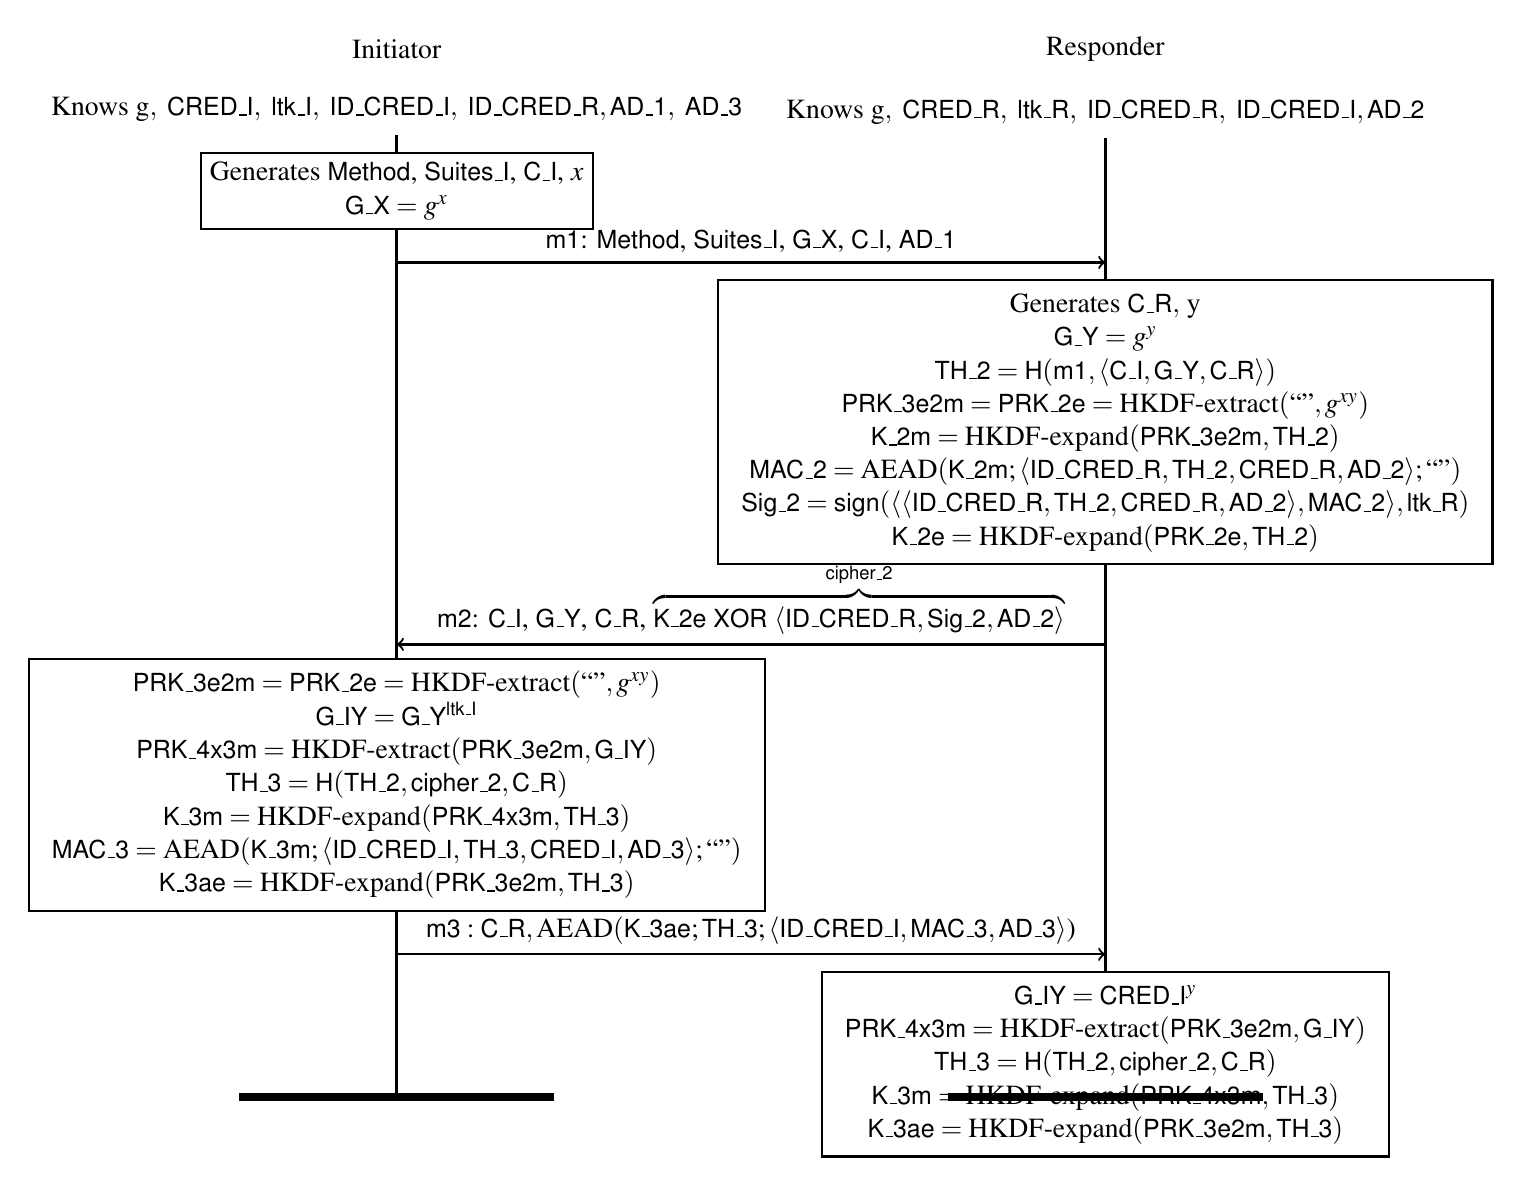
\begin{tikzpicture}
    \node (ini) at (0, 0) {Initiator};
    \draw [very thick] (0, -0.5) -- (0,-13.3);
    \draw [very thick] (9, -0.5) -- (9,-13.3);
    \node[below=0.5em of ini,fill=white,text=black] {$
    \begin{array}{c}
    \text{Knows}\ $g$,\ \mCredi,\ \mLtki,\ \mIdcredi,\ 
    \mIdcredr, \mADone,\ \mADthree
    \end{array}
    $};
    \node (res) at (9,0) {Responder};
    \node[below=0.5em of res,fill=white] {$
    \begin{array}{c}
    \text{Knows}\ $g$,\ \mCredr,\ \mLtkr,\ \mIdcredr,\
    \mIdcredi, \mADtwo
    \end{array}$};
    \action{3em}{ini}{Generates \mMethod,\ \mSuites,\ \mCi,\ $x$\\$\mGx = g^{x}$};
    \msg{7em}{ini}{res}{\mMsgone: \mMethod, \mSuites, \mGx, \mCi, \mADone};
    \action{7.5em}{res}{$
      \begin{array}{c}
        \text{Generates } \mCr,\ $y$\\
        \mGy = g^{y}\\
        \mTHtwo = \mHash(\mMsgone, \langle \mCi, \mGy, \mCr \rangle)\\
        \mPRKthree = \mPRKtwo = \mHkdfExtract(\textrm{``\phantom{}''}, g^{xy}) \\
        \mKtwom = \mHkdfExpand(\mPRKthree, \mTHtwo) \\
        \mMactwo = \mAead(\mKtwom; \langle \mIdcredr, \mTHtwo, \mCredr, \mADtwo \rangle; \textrm{``\phantom{}''}) \\
        \mSigtwo = \mSign(\langle \langle \mIdcredr, \mTHtwo, \mCredr, \mADtwo \rangle, \mMactwo \rangle, \mLtkr)\\
        \mKtwoe = \mHkdfExpand(\mPRKtwo, \mTHtwo)
      \end{array}$};
    \msg{20.7em}{res}{ini}{\mMsgtwo: \mCi, \mGy, \mCr, $\overbrace{\mKtwoe\ \mXor\ \langle \mIdcredr, \mSigtwo, \mADtwo \rangle}^{\mCipher}$};
    \action{21.3em}{ini}{$
      \begin{array}{c}
        \mPRKthree = \mPRKtwo = \mHkdfExtract(\textrm{``\phantom{}''}, g^{xy}) \\
        \mGiy = \mGy^{\mLtki} \\
        \mPRKfour = \mHkdfExtract(\mPRKthree, \mGiy) \\
        \mTHthree = \mHash(\mTHtwo, \mCipher, \mCr)\\
        \mKthreem = \mHkdfExpand(\mPRKfour, \mTHthree) \\
        \mMacthree = \mAead(\mKthreem; \langle \mIdcredi, \mTHthree, \mCredi, \mADthree \rangle; \textrm{``\phantom{}''}) \\
        \mKthreeae = \mHkdfExpand(\mPRKthree, \mTHthree) \\
      \end{array}$};
    \msg{32em}{ini}{res}{$\mMsgthree: \mCr, \mAead(\mKthreeae; \mTHthree; \langle \mIdcredi, \mMacthree, \mADthree \rangle$)};
    \action{32.5em}{res}{$
    \begin{array}{c}
       \mGiy = \mCredi^{y} \\
       \mPRKfour = \mHkdfExtract(\mPRKthree, \mGiy) \\
       \mTHthree = \mHash(\mTHtwo, \mCipher, \mCr)\\
        \mKthreem = \mHkdfExpand(\mPRKfour, \mTHthree) \\
        \mKthreeae = \mHkdfExpand(\mPRKthree, \mTHthree)
    \end{array}$};
    \draw [line width=1mm] (-2,-13.3) -- (2,-13.3);
    \draw [line width=1mm] (7,-13.3) -- (11,-13.3);
    \end{tikzpicture}}
\caption{The \mStatSig{} method of \mEdhoc. \mCredr{} and \mLtkr{} must be signature keys.}
\label{fig:edhocstatsig}
\end{figure}


\fi

\end{document}
